\chapter{Quality Classification System}\label{ch:quality-classification-system}

The original idea was to leverage some Machine Learning classification algorithm to automatically classify datasets.
During thesis elaboration the referential materials turned out to be insufficient in providing usefull information on the topic, hence different technique was chosen (composite statistical score-card evaluation).
Shortcoming of white-papers about Machine Learning supported DQ classification probably results from the absence of well-defined general DQA algorithm and output classes.
Complexity of developing all-embracing method for DQA competes with unfolding general artificial intelligence, indeed.

\section{Data Quality Dimensions}

% Tabular vs relational data
% Tabular data structures: Cross-Sectional, Time-Series, Pooled Cross-Sections, Panel (Longitudal)
% Metrics usability with raw (non-aggregated) and aggregated data.

In order to provide an objective way to measure data quality, we have to choose some DQ metrics and define formal way to compute them.
The list of all candidates can be seen in the Figure~\ref{fig:dq-criteria}.
Many of these candidates are very suitable for specific cases, but completely inappropriate for general use.
After narrowing the selection due to general applicability, we get this list of metrics: completeness, uniqueness, timeliness, validity, accuracy and consistency~\cite{ehdi2019}.

\subsection{Uniqueness}

Uniqueness indicates that each data record should be unique, or else the risk of accessing obsolete information rises.
Just one instance of each real-world object should be recorded in a dataset.
We may have two rows with objects \enquote{John Doe} and \enquote{Jonathan Doe}, who are the same person, but the latter has the most up-to-date information.
Any metrics involving those object instances (e.g., customer count, average spend per customer and sales frequency) would return incorrect results.
Identifying a suitable primary key is the first step in resolving this issue.
In the example, having different names and Customer IDs, but matching email addresses is a good indicator that they are in fact the same individual.
This means that before any analysis or modeling, an additional phase of data inspection is required to consolidate these records.

Leveraging information theory enables us to move the idea forward.
The supporting method for calculating uniqueness could be the calculation of entropy for each record and comparison through distance statistics~\cite{venkatesh2010}.
For each key, we could compute the Shannon entropy \( H \) of the values.
The higher the entropy, the more diverse the key's values are.
Entities with similar entropy are likely to be the same objects.

\subsection{Validity}

Validiy is a quality dimension that refers to information that does not obey business standards or conforms to a particular format.
For example, surname must be a sequence of alphabetic characters and telephone numbers must be composed of numeric characters and must comply with specific regional rules.
Regular expressions can be used to check for validity in a variety of contexts.
Databases containing regular expressions for many common data types are available online.
For discrete data types, simple frequency statistics can tell whether there is a validity issue (e.g., school grades data type with more than 4-5 elements).
It basically becomes a completeness problem once invalid data is found.

\subsection{Accuracy}

Accuracy shows how reliable the data reflect the object or event in the real world.
For example, if a temperature in the room is 21°C, but the thermometer says it is 25°C, that information is inaccurate.
Probably the easiest way to improve accuracy is to introduce redundancy into the system.
An additional check of the acquired data will help to identify discrepancies before entering the system.

\subsection{Completeness}

Blake and Mangiameli (2011) defined completeness as follows.
On the level of data values, a~data value is incomplete (i.e., the metric value is zero) if and only if it is \enquote*{NULL}, otherwise it is complete (i.e., the metric value is one).
A tuple in a relation is defined as complete if all data values are complete (i.e., none of its data values is \enquote*{NULL}).
For a relation \( R \), let \( T_R \) be the number of tuples in \( R \) which have at least one \enquote*{NULL}-value and let \( N_R \) be the total number of tuples in \( R \). Then, the completeness \( C \) of \( R \) is defined as follows~\cite{blake2011}.

\begin{equation}
    C = 1 - \frac{T_R}{N_R} = \frac{N_R - T_R}{N_R}
\end{equation}

This definition of \textit{completeness} meets the requirements for metrics according to Heinrich et al. (2018).
The metric values are within the bounded interval \( \left[0; 1\right] \) for all aggregation levels.
The minimum value represents perfectly poor data quality and vice versa.
To archieve full score, no tuple must not contain a null value, as well as relations must not contain any tuple with data values which equal \enquote*{NULL}.

The metric is reliable because all configuration parameters of the metric can be determined by a database query.
Due to the existence of a mathematical formula, the metric is objective and because the metric quantifies a dimension at all quality levels according to the corresponding definition, the determination of the metric value is also valid.
The metric formula is applicable to single data values as well as to sets of data values.

\subsection{Consistency}

There are several forms of data consistency.
The \textbf{first form} is actual wide or narrow distribution of data.
In this way, consistency of data can be viewed as \textit{stability}, \textit{uniformity} or \textit{constancy}.

\begin{figure}[htb]
    \centering
    
    \begin{equation*}
        \sigma = \sqrt{\frac{1}{N}\sum_{i=1}^{N} (x_{i} - \mu)^2}
    \end{equation*}

    \caption{Population Standard Deviation formula}
    \label{form:population-standard-dev}
\end{figure}
\FloatBarrier

Typical measures include statistics such as the \textit{range} (i.e., the largest value minus the smallest value among a distribution of data), the \textit{variance} (i.e., the sum of the squared deviations of each value in a distribution from the mean value in a distribution divided by the number of values in a distribution) and the \textit{standard deviation} (i.e., the square root of the variance).

\begin{figure}[htb]
    \centering
    
    \begin{equation*}
        s = \sqrt{\frac{1}{N - 1}\sum_{i=1}^{N} (x_{i} - \bar{x})^2}
    \end{equation*}

    \caption{Sample Standard Deviation formula}
    \label{form:sample-standard-dev}
\end{figure}
\FloatBarrier

If one is evaluating the consistency of data drawn in a sample from a population, the \textit{standard error of the mean} (i.e., the standard deviation of the sampled population divided by the square root of the sample size) is often examined.
Finally, the constancy of data produced by instruments and tests is typically measured by estimating the reliability of~obtained scores.
Reliability estimates include test-retest coefficients, split-half measures and Kuder-Richardson Formula \textnumero 20 indexes~\cite{quora:consistency2017}.
For Time Series data, stationary analysis can be done.
If the data is non-stationary then it is likely to have some degree of inconsistency.

\begin{figure}[htb]
    \centering
    
    \begin{equation*}
        \sigma_{\bar{x}} = \frac{\sigma}{\sqrt{n}}
    \end{equation*}

    \caption{Standard Error of the Mean formula}
    \label{form:sem}
\end{figure}
\FloatBarrier

Then, there is \textbf{second form} of data consistency; whether data are uniformly defined throughout the dataset, that is, across variables and over time.
For example, suppose we want to use the data to estimate real estate sales per year to see how that number has changed over time.
In this case, we have to make sure the estimates of real estate sales are uniformly defined over time.
Specifically, does the data series always either include apartments or exclude apartments from the counts?
Does it always either include houses or exclude houses from the counts?
If the data sometimes include apartments, but not always, or if the data sometimes include houses, but not always, then the data are inconsistent.

The \textbf{third form} of consistency tightly coupled with relational databases and their referential integrity.
A relational database is said to be ACID (vs non-relational BASE), meaning
\begin{enumerate*}[label=(\roman*)]
    \item atomicity,
    \item consistency,
    \item isolation and
    \item durability.
\end{enumerate*}
The term onsistency there refers to the requirement that any given database transaction must affect data only in allowed ways, therefore data must be valid according to all defined rules, including constraints, cascades, triggers, and any combination thereof.

Inconsistencies in data can be due to changes over time and/or across variables for example, in
\begin{enumerate*}[label=(\roman*)]
    \item vintages or time periods,
    \item units,
    \item levels of accuracy,
    \item levels of completeness,
    \item inclusions and exclusions.
\end{enumerate*}
Those inconsistencies occur most often when merging or aggregating datasets, therefore the user has to make sure data are consistently defined throughout.

\subsection{Timeliness}

Timeliness is another one of the major dimensions in the field of data quality.
Obsolete data suppress innovation, therefore businesses and startups want to trust the data publisher that the data will remain available and relevant, especially when using open data or reference data from central registers.
A measure of timeliness has to focus on the update cycle.
Automation must be a key part of this process, leading to the efficiency in publishing and processing of data.
Meeting all these points is a necessary, but not sufficient condition to create a sustainable data ecosystem.

Atz (2014) proposed an unique metric for measuring the timeliness of data.
The research defines timely dataset as a product of function of the forecast update frequency (a dataset released annualy will be updated only once a year)~\cite{atz2014tau}.
The concept of timeliness \( T \) can be expressed by the equation~\ref{eq:timeliness}.

\begin{equation}\label{eq:timeliness}
    T = I \frac{f_U}{today - last update}
\end{equation}

In the equation~\ref{eq:timeliness}, the \( I \) is an indicator function causing \textit{Heaviside} step function effect returning 1 when the ratio is greater than one and 0 otherwise.
For example, a~dataset with a daily cycle and a last major update last month would result in a 0.
On the other hand, a dataset with monthly cycle and an update in last two weeks, would yield 1.
In the equation \( f_U \) represents \textit{update frequency}; the terms \textit{today} and \textit{last update} are timepoints corresponding to the names.

% Důvod přítomnosti indikátorové funkce je ten, že nemáme nástroj, kterým bychom zhodnotili způsob stárnutí datasetu.
The reason for the presence of the indicator function is that we do not have a tool to evaluate the aging of the dataset.
% Data mohou zastarávat lineárně a spojitě, ale také nelineárně a nespojitě.
Data can become obsolete linearly and continuously, but also non-linearly and discontinuously.
% Tato funkční závislost je nám skryta, data považujeme tedy buď za aktuální nebo zastaralá.
This functional dependence is hidden from us, so we consider the data to be either current or obsolete.

% \[ T = \begin{cases} 0 & x\leq 0 \\ \frac{100-x}{100} & 0\leq x\leq 100 \\ 0 & 100\leq x \end{cases} \]

Atz (2014) introduced a metric for measuring data catalogue timeliness, \( \tau \) (equation~\ref{eq:tau}).
In general, minor changes such as typo correction should not be considered as an update.

\begin{equation}\label{eq:tau}
    \tau = \frac{1}{N} \sum_{i = 1}^N I \left( \frac{f_{U_i} \cdot \lambda + \delta}{today - {last update}_i} \right)
\end{equation}

The \( \tau \) of a data catalogue is the average across datasets, indicated by the subscript \textit{i}~\cite{atz2014tau}.
The number of datasets in the catalog is denoted by the \textit{N}.

Two parameters in a linear form have been introduced to the core of the expression.
The lambda (\( \lambda \)) is degree of freedom relative to the update frequency; the days we allow the update of the data catalog.
For example, considering 5\% of the time reserve (e.g., due to ETL delays), the annual renewal dataset is going have a buffer of 0.6 months and for a monthly dataset it implies 1.5 days in tolerance.
The delta (\( \delta \)) is a fixed number of days applicable to all datasets, for example one day for processing~\cite{atz2014tau}.

\begin{table}[htbp]
    \centering

    \begin{tabular}{@{}ll@{}}
        \toprule
        \( \tau \)  & Data Timeliness   \\ \midrule
        0.9-1       & exemplar          \\
        0.7-0.9     & standard          \\
        0.5-0.7     & ok                \\
        0.25-0.5    & poor              \\
        0-0.25      & obsolete          \\
        \bottomrule
    \end{tabular}

    \caption{Proposed benchmarks for different levels of \( \tau \)~\cite{atz2014tau}}
    \label{table:timeliness-benchmarks}
\end{table}
\FloatBarrier

The trivial case (only one dataset in the catalog) is constrained, by design, to a binary classification, data are either up-to-date or not.
This means that a data catalogue that is one day late is considered the same as one that fails to fully update the datasets.
However, the advantages of simplicity outweigh the disadvantages of a~more complex method.

\section{Weighted Aggregation}

Probably the best known project dealing with data classification is \enquote{5-star Open Data}.
This classification system defines quality in terms of how well they provide the context in which the data is located as well as in how well machine-readable the data is~\cite{w3org5stardata}.
% Data nejvyšší kvality jsou ta, která mají plně definovanou ontologii a jsou propojena s dalšími datasety.
The highest quality data are those that have a fully defined ontology and are connected to other datasets~\cite{5stardata}.
% Pro tento případ se využívá schéma RDF a jazyk SPARQL.
The RDF schema and the SPARQL language are used for this case~\cite{5stardata}.
% Automatickou klasifikaci datasetu lze provést testem existence hypertextových odkazů.
Automatic classification of a dataset can be performed by testing the existence of hyperlinks.
% Využití tohoto frameworku je v kontextu internetu, není tedy pro náš účel příliš vhodný.
The use of this framework is in the context of the Internet, so it is not very suitable for our purpose.

Considering that we want to achieve the relative objectivity of the framework, we will have to use the general metrics discussed in the previous section.
The resulting system should therefore be similar to machine learning ensemble voting.
A Regression Voting Ensemble is a machine learning model that combines the average predictions of contributing models to improve model performance.
Model is shown in the picture~\ref{fig:voting}.

\begin{figure}[htb]
    \centering
    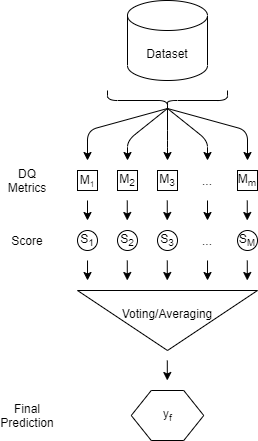
\includegraphics[width=0.4\textwidth]{figures/voting.png}
    \caption{Voting Model}
    \label{fig:voting}
\end{figure}
\FloatBarrier

The model can be expressed using the equation~\ref{eq:voting-model}.

\begin{equation}\label{eq:voting-model}
    y_f = \sum_{i = 1}^{N} w_i y_i
\end{equation}

In the following chapter, we will use this concept as a base to evaluate the performance of the data catalog.

\section{Data Quality Framework Evaluation Instrument}

The Data Quality Framework Evaluation Instrument is a tool developed by Long et al. (2004).
The instrument's primary goal is to promote continuous data quality enhancement and the user limitations tracking~\cite{long2004}.
The instrument is structured as a four-level conceptual framework, with 89 requirements at its root~\cite{long2004}.
Using the instrument algorithm, the criteria can be folded into the second level of 24 data quality characteristics which can then be rolled up into 6 data quality dimensions~\cite{long2004}.
The five dimensions can be combined into a single overall data collection evaluation~\cite{long2004}.
The instrument is designed for the evaluation of medical datasets, we will try to use it unchanged for COVID-19 datasets.

\subsection{Instrument Usage}

Each of the 89 criteria is meant to be scored as \enquote{unknown (0)}, \enquote{not met (2)}, or \enquote{met (3)}~\cite{long2004}.
Each score must be briefly substantiated in writing.
All dimensions are scored as \enquote{unknown (0)}, \enquote{not acceptable (1)}, \enquote{marginal (2)}, and \enquote{appropriate (3)}~\cite{long2004}.

Long et al. (2004) proposed the following procedure for aggregating criteria into characteristics.
\begin{enumerate}
    \item If one of the criteria within a characteristic is \enquote{unknown} then the characteristic is scored as \enquote{unknown}~\cite{long2004}.
    \item If the status of all the criteria is known and more than half are \enquote{not acceptable} then the characteristic is \enquote{not acceptable}~\cite{long2004}.
    \item If the status of all the criteria is known and half are \enquote{met} then the characteristic is scored as \enquote{marginal}~\cite{long2004}.
    \item If all the criteria are \enquote{met} then the characteristic is \enquote{appropriate}~\cite{long2004}.
\end{enumerate}

\noindent The procedure for characteristic-dimensions aggregation is as follows.
\begin{enumerate}
    \item If one of the characteristics within a dimension is \enquote{unknown} then the dimension is scored as \enquote{unknown}~\cite{long2004}.
    \item If the status of all the characteristics is known and at least one is \enquote{not acceptable} then the dimension is \enquote{not acceptable}~\cite{long2004}.
    \item If the status of all the characteristics is known and they are a combination of \enquote{marginal} and \enquote{appropriate} then the dimension is scored as \enquote{marginal}~\cite{long2004}.
    \item If all the characteristics are \enquote{appropriate}, then the dimension is \enquote{appropriate}~\cite{long2004}.
\end{enumerate}

The algorithm proposed by the authors of the article is suitable for datasets which we have complete information about.
However, this will not be our case.
There will be too many questions that we cannot answer directly in the questionnaire.
This would probably lead to a final evaluation of the dimensions as unknown.
The algorithm also assumes that all dimensions, characteristics, and criteria have the same weight, which generally may not be the case.

\subsection{Conclusion}

The advantage of the presented approach is that it can be used both for individual data sets and for the data catalog.
The disadvantage of the approach is that the evaluation of criteria in a more specialized field will require the cooperation of industry and IT specialists.
The main limitation is that the questions in the questionnaire provide only a vague idea of the state of the data in the database (e.g., integrity).
On the other hand, they provide a comprehensive overview of the status of data, including the process of data collection and staff training.
Fortunately, this condition is suitable for the COVID-19 dataset.

Additional criteria can be added to the questionnaire.
However, such an intervention requires a field specialist and subsequent testing of the evaluation process.
